% This is text associated with the open textbook "Open Electromagnetics"
% See immediately below for author, date
% This work is licensed under the Creative Commons Attribution-ShareAlike 4.0 International License. (CC BY SA 4.0) 
% To view a copy of the license, visit http://creativecommons.org/licenses/by-sa/4.0/

%ORB TITLE Torque Induced by a Magnetic Field
%ORB AUTHOR 0        # S.W. Ellingson, Virginia Tech (ellingson@vt.edu)
%ORB DATE 20191117   # yyyymmdd
%ORB ABSTRACT 

\label{m0024_Torque_Induced_by_a_Magnetic_Field} % <-- Must match name of this file and module directory name.  Don't mess with this!

A magnetic field exerts a force on current.  
This force is exerted in a direction perpendicular to the direction of current flow.  
For this reason, current-carrying structures in a magnetic field tend to rotate.  
A convenient description of force associated with rotational motion is \emph{torque}.
\index{torque}
In this section, we define torque and apply this concept to a closed loop of current.
These concepts apply to a wide range of practical devices, including electric motors.   

Figure~\ref{m0024_fTorque} illustrates the concept of torque.
%
\begin{figure}[b!]
\begin{center}
\pdftooltip{{  % note double braces
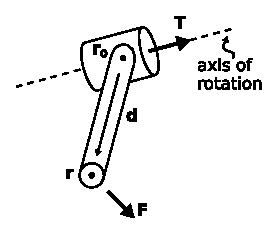
\includegraphics[width=0.8\columnwidth]{modules/m0024_fTorque.eps} 
}}{Torque, capital T, being generated in a cylindrical object by applying force on a single lever arm connected to the object. Lever arm labeled small d with the axis of rotation labeled small r subscript 0, and opposite end labeled small r. Force, capital F, is applied to the lever arm at point small r.}
\end{center}
\centerline{\scriptsize 
\copyright~\hyperref[m0024_fTorque_Credit]{C.\ Wang} 
\href{https://creativecommons.org/licenses/by-sa/4.0/}{CC BY-SA 4.0} 
} 
\caption{
\label{m0024_fTorque}
Torque associated with a single lever arm.
}
\end{figure}
%
Torque depends on the following:
%
\begin{itemize}
\item A local origin ${\bf r}_0$,
\item A point {\bf r} which is connected to ${\bf r}_0$ by a perfectly-rigid mechanical structure, and
\item The force ${\bf F}$ applied at ${\bf r}$. 
\end{itemize}
In terms of these parameters, the torque ${\bf T}$ is:
%
\begin{equation}
{\bf T} \triangleq {\bf d} \times {\bf F}
\end{equation}
%
where the \emph{lever arm}
\index{lever arm}
${\bf d} \triangleq {\bf r} - {\bf r}_0$ gives the location of ${\bf r}$ relative to ${\bf r}_0$.
Note that ${\bf T}$ is a position-free vector 
\index{vector!position-free}
which points in a direction perpendicular to both ${\bf d}$ and ${\bf F}$.
  
Note that ${\bf T}$ does not point in the direction of rotation.
Nevertheless, ${\bf T}$ indicates the direction of rotation through a ``right hand rule'':  If you point the thumb of your right hand in the direction of ${\bf T}$, then the curled fingers of your right hand will point in the direction of torque-induced rotation.

Whether rotation actually occurs depends on the geometry of the structure. 
For example, if ${\bf T}$ aligns with the axis of a perfectly-rigid mechanical shaft, then all of the work done by ${\bf F}$ will be applied to rotation of the shaft on this axis.
Otherwise, torque will tend to rotate the shaft in other directions as well.
If the shaft is not free to rotate in these other directions, then the \emph{effective torque} -- that is, the torque that contributes to rotation of the shaft -- is reduced.

The magnitude of ${\bf T}$ has SI base units of N$\cdot$m and quantifies the energy associated with the rotational force.
As you might expect, the magnitude of the torque increases with increasing lever arm magnitude $\left|{\bf d}\right|$.
In other words, the torque resulting from a constant applied force increases with the length of the lever arm.

Torque, like the translational force {\bf F}, satisfies superposition.  
That is, the torque resulting from forces applied to multiple rigidly-connected lever arms is the sum of the torques applied to the lever arms individually.

Now consider the current loop shown in Figure~\ref{m0024_fCurrentLoop}.
The loop is perfectly rigid and is rigidly attached to a non-conducting shaft.
The assembly consisting of the loop and the shaft may rotate without friction around the axis of the shaft.
The loop consists of four straight segments that are perfectly-conducting and infinitesimally-thin.
A spatially-uniform and static impressed magnetic flux density ${\bf B}_0 = \hat{\bf x} B_0$ exists throughout the domain of the problem.
(Recall that an \emph{impressed} field is one that exists in the absence of any other structure in the problem.)
What motion, if any, is expected?
%
\begin{figure}[b!]
\begin{center}
\pdftooltip{{  % note double braces
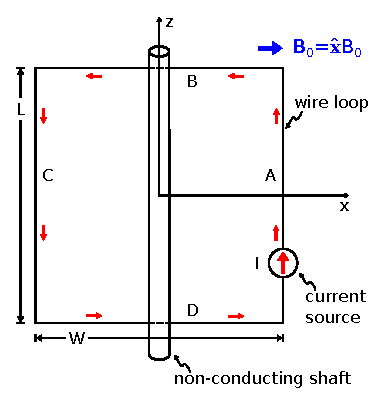
\includegraphics[width=0.8\columnwidth]{modules/m0024_fCurrentLoop.eps} 
}}{On an x-z coordinate system sits a square wire loop centered at the origin. The right side of the square loop is labeled capital A, the top is labeled B, the left is labeled C, and the bottom is labeled D with current source capital I on segment A and moving counter-clockwise through the loop. The height of the loop is capital L and the width is capital W. The non-conducting shaft of motor is centered and runs vertically along the z axis. Above motor reads boldface capital B sub 0 equals boldface x hat boldface capital B sub 0.}
\end{center}
\centerline{\scriptsize 
\copyright~\hyperref[m0024_fCurrentLoop_Credit]{C.\ Wang} 
\href{https://creativecommons.org/licenses/by-sa/4.0/}{CC BY-SA 4.0} 
} 
\caption{
\label{m0024_fCurrentLoop}
A rudimentary electric motor consisting of a single current loop.
}
\end{figure}

Recall that the net translational force on a current loop in a spatially-uniform and static magnetic field is zero (Section~\ref{m0017_Magnetic_Force_Current-Carrying_Wire}).
However, this does not preclude the possibility of different translational forces acting on each of the loop segments resulting in a rotation of the shaft.
Let us first calculate these forces.
The force ${\bf F}_A$ on segment~A is 
%
\begin{equation}
{\bf F}_A = I{\bf l}_A \times {\bf B}_0 
\end{equation}
%
where ${\bf l}_A$ is a vector whose magnitude is equal to the length of the segment and which points in the direction of the current. Thus,
%
\begin{flalign}
{\bf F}_A &= I\left(\hat{\bf z}L\right) \times \left( \hat{\bf x}B_0 \right) \nonumber \\
          &= \hat{\bf y}ILB_0
\end{flalign}
%
Similarly, the force ${\bf F}_C$ on segment~C is
%
\begin{flalign}
{\bf F}_C &= I\left(-\hat{\bf z}L\right) \times \left( \hat{\bf x}B_0 \right) \nonumber \\
          &= -\hat{\bf y}ILB_0
\end{flalign}
%
The forces ${\bf F}_B$ and ${\bf F}_D$ on segments~B and D, respectively, are:
%
\begin{equation}
{\bf F}_B = I\left(-\hat{\bf x}L\right) \times \left( \hat{\bf x}B_0 \right) = 0 
\end{equation}
and
%
\begin{equation}
{\bf F}_D = I\left(+\hat{\bf x}L\right) \times \left( \hat{\bf x}B_0 \right) = 0 
\end{equation}
%
Thus, the force exerted on the current loop by the impressed magnetic field will lead to rotation in the $+\hat{\bf \phi}$ direction.

We calculate the associated torque ${\bf T}$ as 
%
\begin{equation}
{\bf T} = {\bf T}_A + {\bf T}_B + {\bf T}_C + {\bf T}_D 
\end{equation}
%
where ${\bf T}_A$, ${\bf T}_B$, ${\bf T}_C$, and ${\bf T}_D$ are the torques associated with segments~A, B, C, and D, respectively.
For example, the torque associated with segment~A is
%
\begin{flalign}
{\bf T}_A &= \frac{W}{2}\hat{\bf x} \times {\bf F}_A \nonumber \\
          &= \hat{\bf z}L\frac{W}{2}IB_0 
\end{flalign}
%
Similarly,
%
\begin{equation}
{\bf T}_B = 0 ~\mbox{since ${\bf F}_B=0$} 
\end{equation}
%
\begin{equation}
{\bf T}_C = \hat{\bf z}L\frac{W}{2}IB_0 
\end{equation}
%
\begin{equation}
{\bf T}_D = 0 ~\mbox{since ${\bf F}_D=0$} 
\end{equation}
%
Summing these contributions, we find
%
\begin{equation}
{\bf T} = \hat{\bf z}LWIB_0 
\end{equation}
%
Note that ${\bf T}$ points in the $+\hat{\bf z}$ direction, indicating rotational force exerted in the $+\hat{\bf \phi}$ direction, as expected.
Also note that the torque is proportional to the area $LW$ of the loop, is proportional to the current $I$, and is proportional to the magnetic field magnitude $B_0$.

The analysis that we just completed was \emph{static}; that is, it applies only at the instant depicted in Figure~\ref{m0024_fCurrentLoop}.
If the shaft is allowed to turn without friction, then the loop will rotate in the $+\hat{\bf \phi}$ direction.
So, what will happen to the forces and torque?
First, note that ${\bf F}_A$ and ${\bf F}_C$ are always in the $+\hat{\bf y}$ and $-\hat{\bf y}$ directions, respectively, regardless of the rotation of the loop.  
Once the loop rotates away from the position shown in Figure~\ref{m0024_fCurrentLoop}, the forces ${\bf F}_B$ and ${\bf F}_D$ become non-zero; however, they are always equal and opposite, and so do not affect the rotation.
Thus, the loop will rotate one-quarter turn and then come to rest, perhaps with some damped oscillation around the rest position depending on the momentum of the loop.
At the rest position, the lever arms for segments~A and C are pointing in the same directions as ${\bf F}_A$ and ${\bf F}_C$, respectively.
Therefore, the cross product of the lever arm and translational force for each segment is zero and subsequently ${\bf T}_A={\bf T}_C=0$.
Once stopped in this position, both the net translational force and the net torque are zero.

If such a device is to be used as a motor,
\index{motor}
it is necessary to find a way to sustain the rotation.
There are several ways in which this might be accomplished.
First, one might make $I$ variable in time.
For example, the direction of $I$ could be reversed as the loop passes the quarter-turn position.
This reverses ${\bf F}_A$ and ${\bf F}_C$, propelling the loop toward the half-turn position.
The direction of $I$ can be changed again as the loop passes half-turn position, propelling the loop toward the three-quarter-turn position.  
Continuing this periodic reversal of the current sustains the rotation.
Alternatively, one may periodically reverse the direction of the impressed magnetic field to the same effect.
These methods can be combined or augmented using multiple current loops or multiple sets of time-varying impressed magnetic fields.
Using an appropriate combination of current loops, magnetic fields, and waveforms for each, it is possible to achieve sustained torque throughout the rotation.
An example is shown in Figure~\ref{m0024_fElectric_motor}.
%
\begin{figure}
\begin{center}
\pdftooltip{{  % note double braces
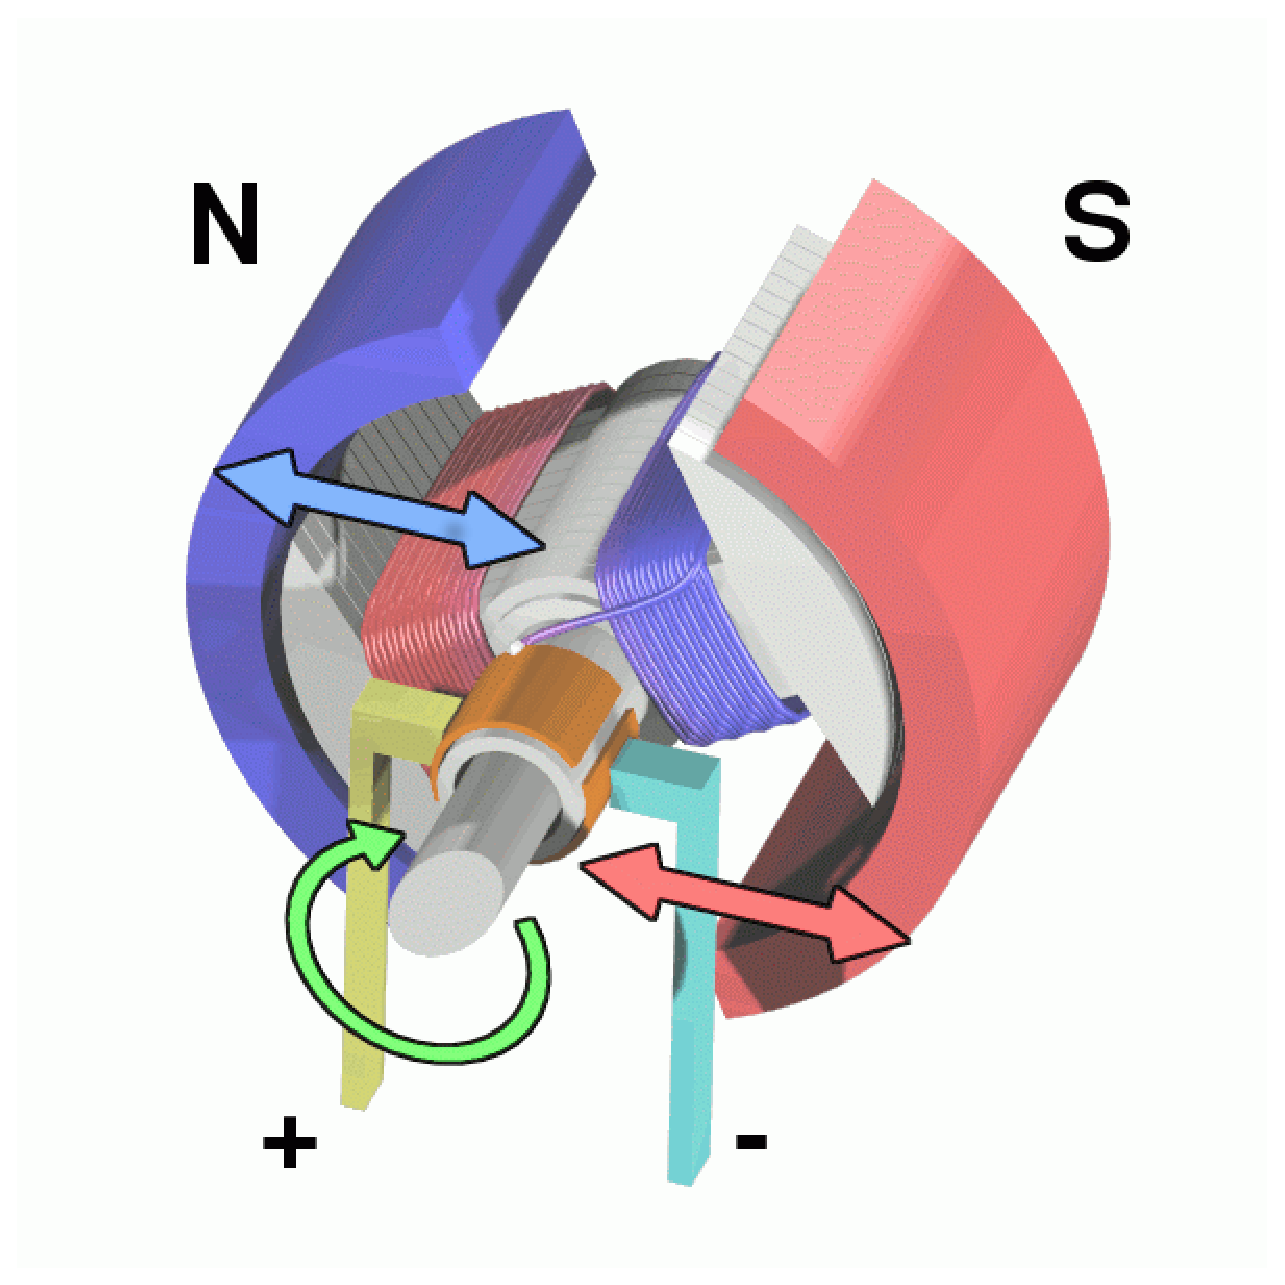
\includegraphics[width=\columnwidth]{modules/m0024_Electric_motor.eps} 
% https://en.wikipedia.org/wiki/File:Electric_motor.gif
}}{A t-shaped object with a cylindrical shaft and bar with rounded ends. The shaft is connected to a positive lead on the left and a negative lead on the right. The shaft rotates clockwise. The shaft is connected to a horizontal bar that is wrapped in red wire (left) and blue wire (right). On the left end of the bar is a brush labeled capital N and on the right end of the bar is a brush labeled capital S.}
\end{center}
\centerline{\scriptsize 
\copyright~\hyperref[m0024_fElectric_motor_Credit]{Abnormaal} 
\href{https://creativecommons.org/licenses/by-sa/3.0/}{CC BY-SA 3.0} 
} 
\caption{
\label{m0024_fElectric_motor}
This DC electric motor uses brushes (here, the motionless leads labeled ``$+$'' and ``$-$'') combined with the motion of the shaft to periodically alternate the direction of current between two coils, thereby creating nearly constant torque.
}
\end{figure}

~\\
%%%%%%%%%%%%%%%%%%%%%%%%%%%

{\bf Additional Reading:}
\begin{itemize}
\item ``\href{https://wikipedia.org/wiki/Torque}{Torque}'' on Wikipedia.
\item ``\href{https://wikipedia.org/wiki/Electric_motor}{Electric motor}'' on Wikipedia.
\end{itemize}

